\subsection{Lab15: Receptor AM}

%*********************
\begin{frame}{}

\pgfdeclareimage[width=\paperwidth,height=\paperheight]{bg}{imagenes/fondo_lab}
\setbeamertemplate{background}{\pgfuseimage{bg}}

\bfseries{\textrm{\LARGE Lab15\\ \Large Receptor AM}}
\raggedright
\end{frame}
%*********************

\begin{frame}{Receptor AM}

\pgfdeclareimage[width=\paperwidth,height=\paperheight]{bg}{imagenes/fondo3}
\setbeamertemplate{background}{\pgfuseimage{bg}}

El funcionamiento de un demodulador IQ se puede explicar representando su señal de entrada de RF $sRF(t)$ como una combinación de dos portadoras de cuadratura modulada de doble banda lateral:

\vspace{3mm}
\begin{center}
    $sRF (t)=S I(t)+S Q(t) = I(t)cos(w RF)t-Q(t)sin(w RF)t$ 
\end{center}

\vspace{2mm}
El componente en fase $I(t)$ y el componente de cuadratura $Q(t)$ son señales de banda base que se pueden ver como entradas a un modulador IQ ideal que genera $1sRF(t)$.
\end{frame}
%---------------------------------

\begin{frame}{Receptor AM}

A continuación, construiremos un receptor de AM simple para la recepción de banda de transmisión y onda corta. En el receptor se utiliza el hardware HackRF. Además, muestra cómo configurar y mostrar la frecuencia del receptor.\vspace{2mm}

El diseño del receptor AM principalmente consta de:

\begin{itemize}
    \item {\textit{Osmocom source} = Fuente HackRF}
    \item {\textit{Low pass filter} = Filtro pasa bajas con frecuencia de corte de 5KHz.}
    \item {\textit{Complex to Mag} = Permite realizar la demodulación de una manera más compleja}
    \item {\textit{Multiply const} = Para tener cierta ganancia}
    \item {\textit{Sumidero de audio Audio Sink} = para poder escuchar la señal demodulada.}
    
\end{itemize}{}

\end{frame}
%---------------------------------

\begin{frame}{Receptor AM}

\begin{figure}[H]
\centering
\vspace{-3mm}
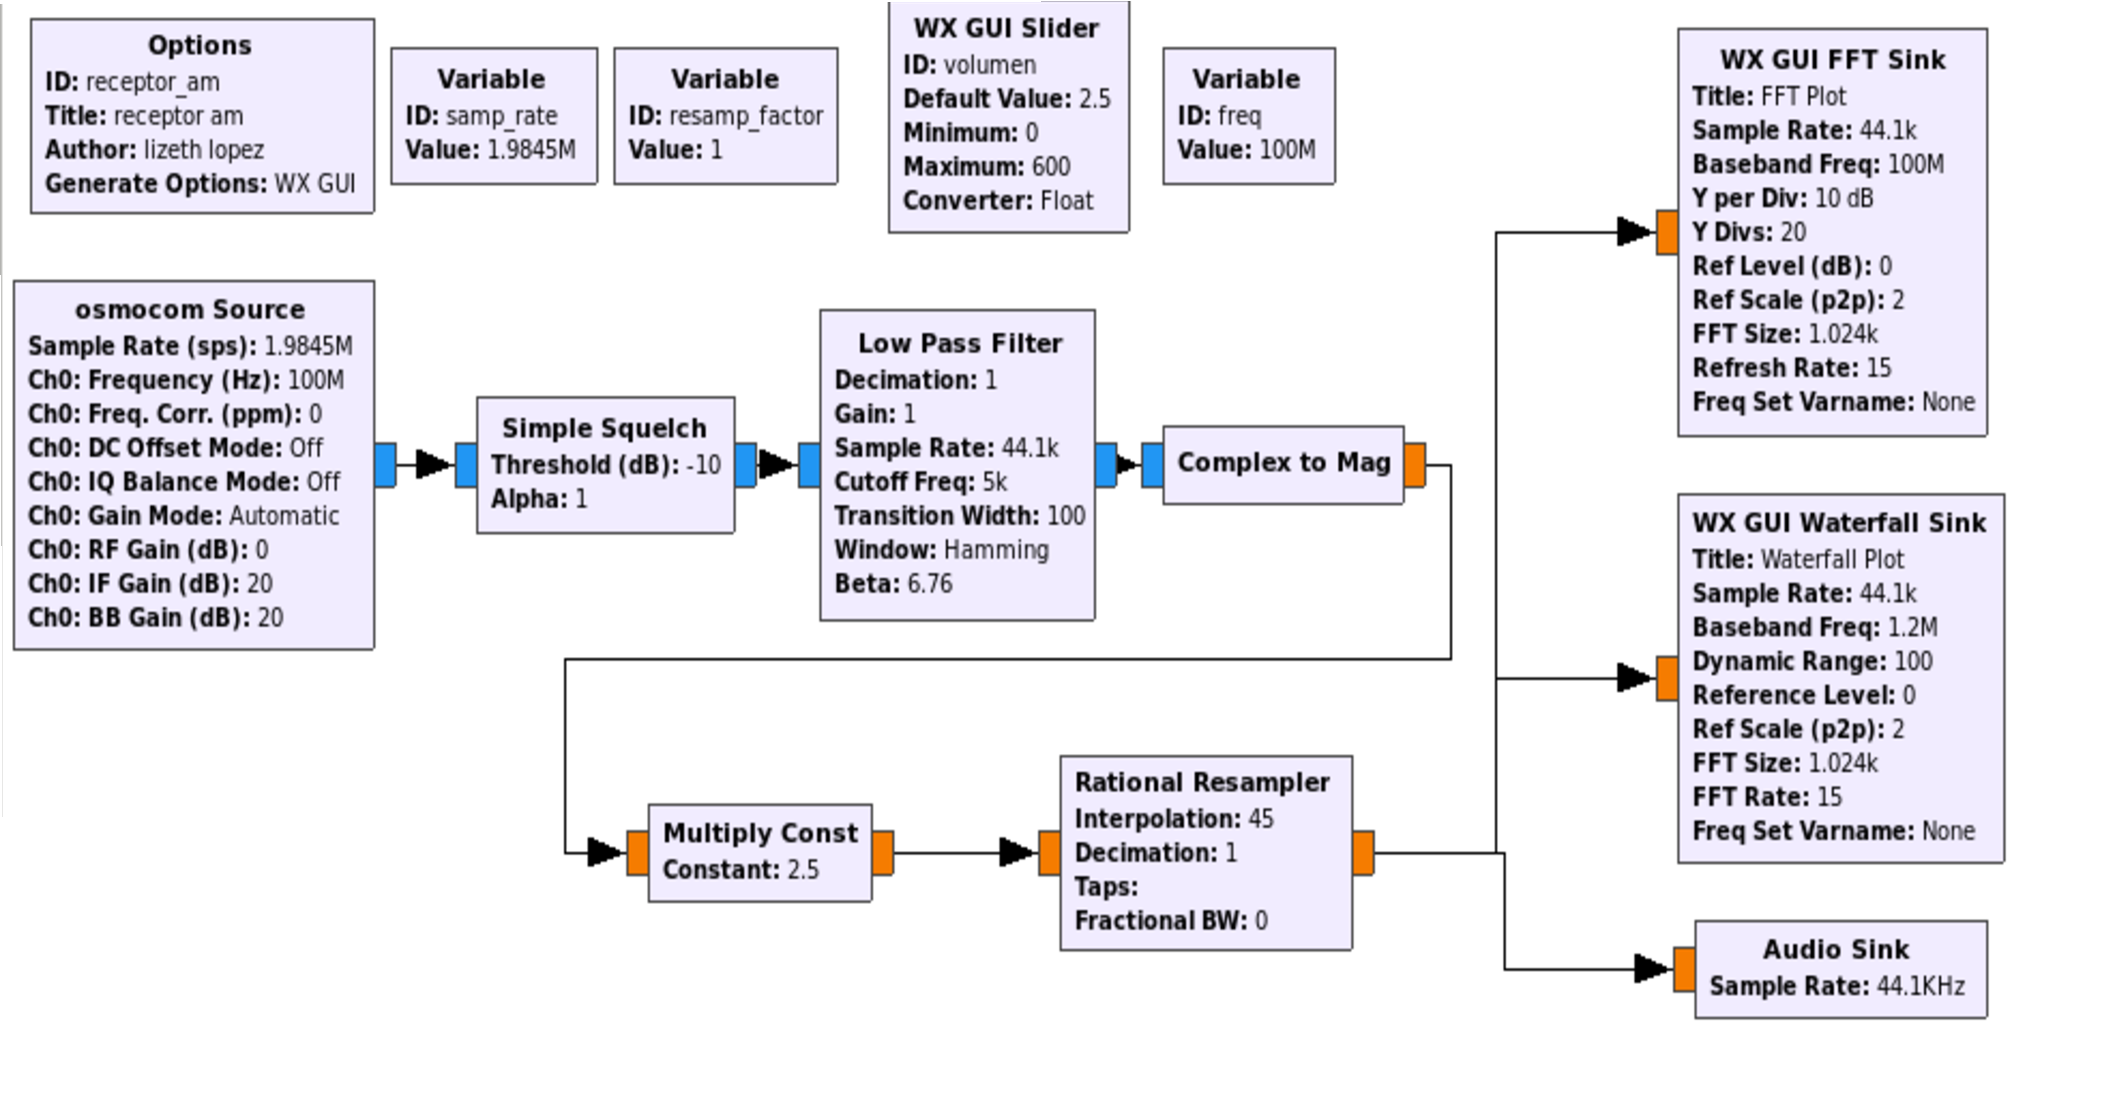
\includegraphics[width=\textwidth]{parte3/lab16/pdf/lab16_1.pdf}
\end{figure}

\end{frame}
%---------------------------------

\begin{frame}{Receptor AM}

\begin{figure}[H]
\centering
\vspace{-3mm}
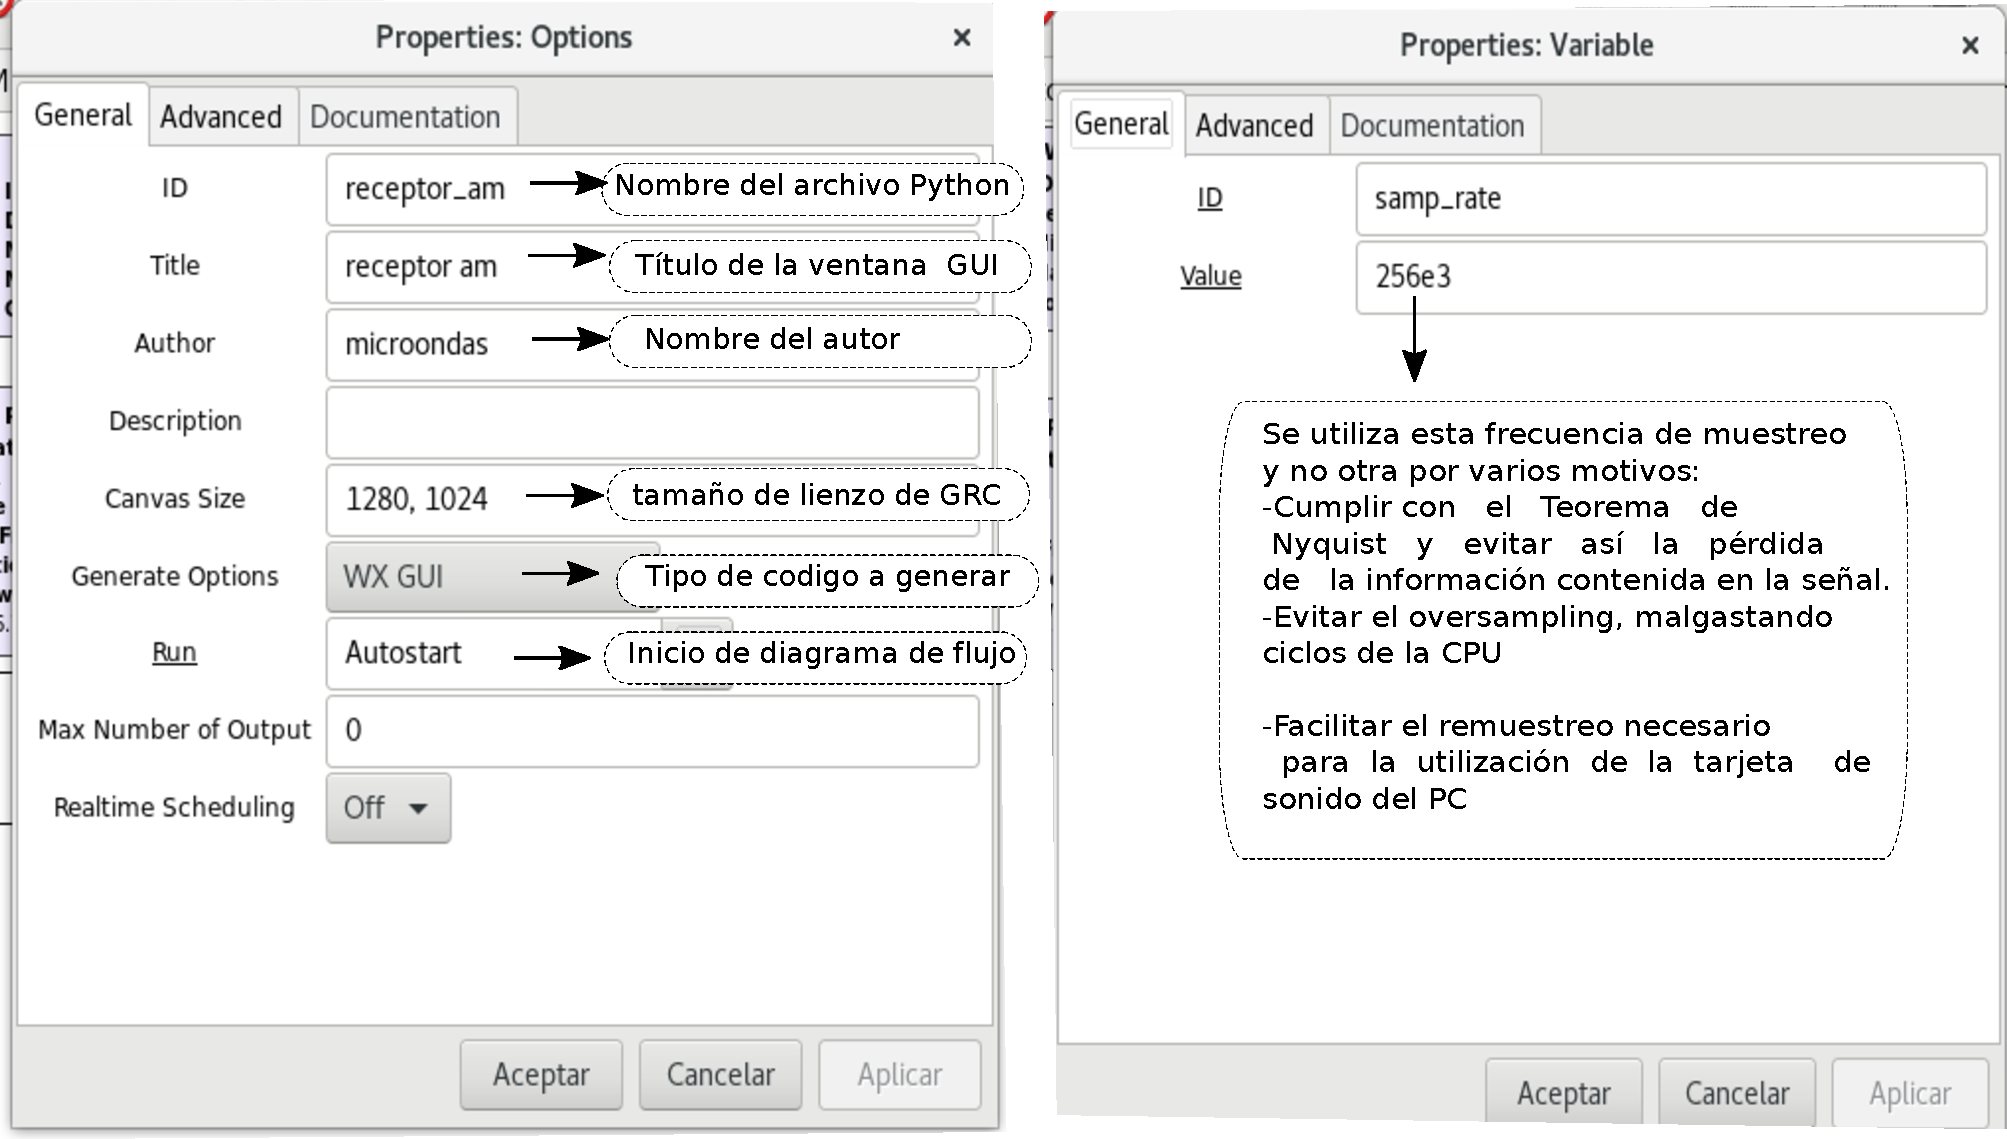
\includegraphics[width=\textwidth]{parte3/lab16/pdf/lab16_2.pdf}

\end{figure}

\end{frame}
%---------------------------------

\begin{frame}{Receptor AM}

\begin{figure}[H]
\centering
\vspace{-3mm}
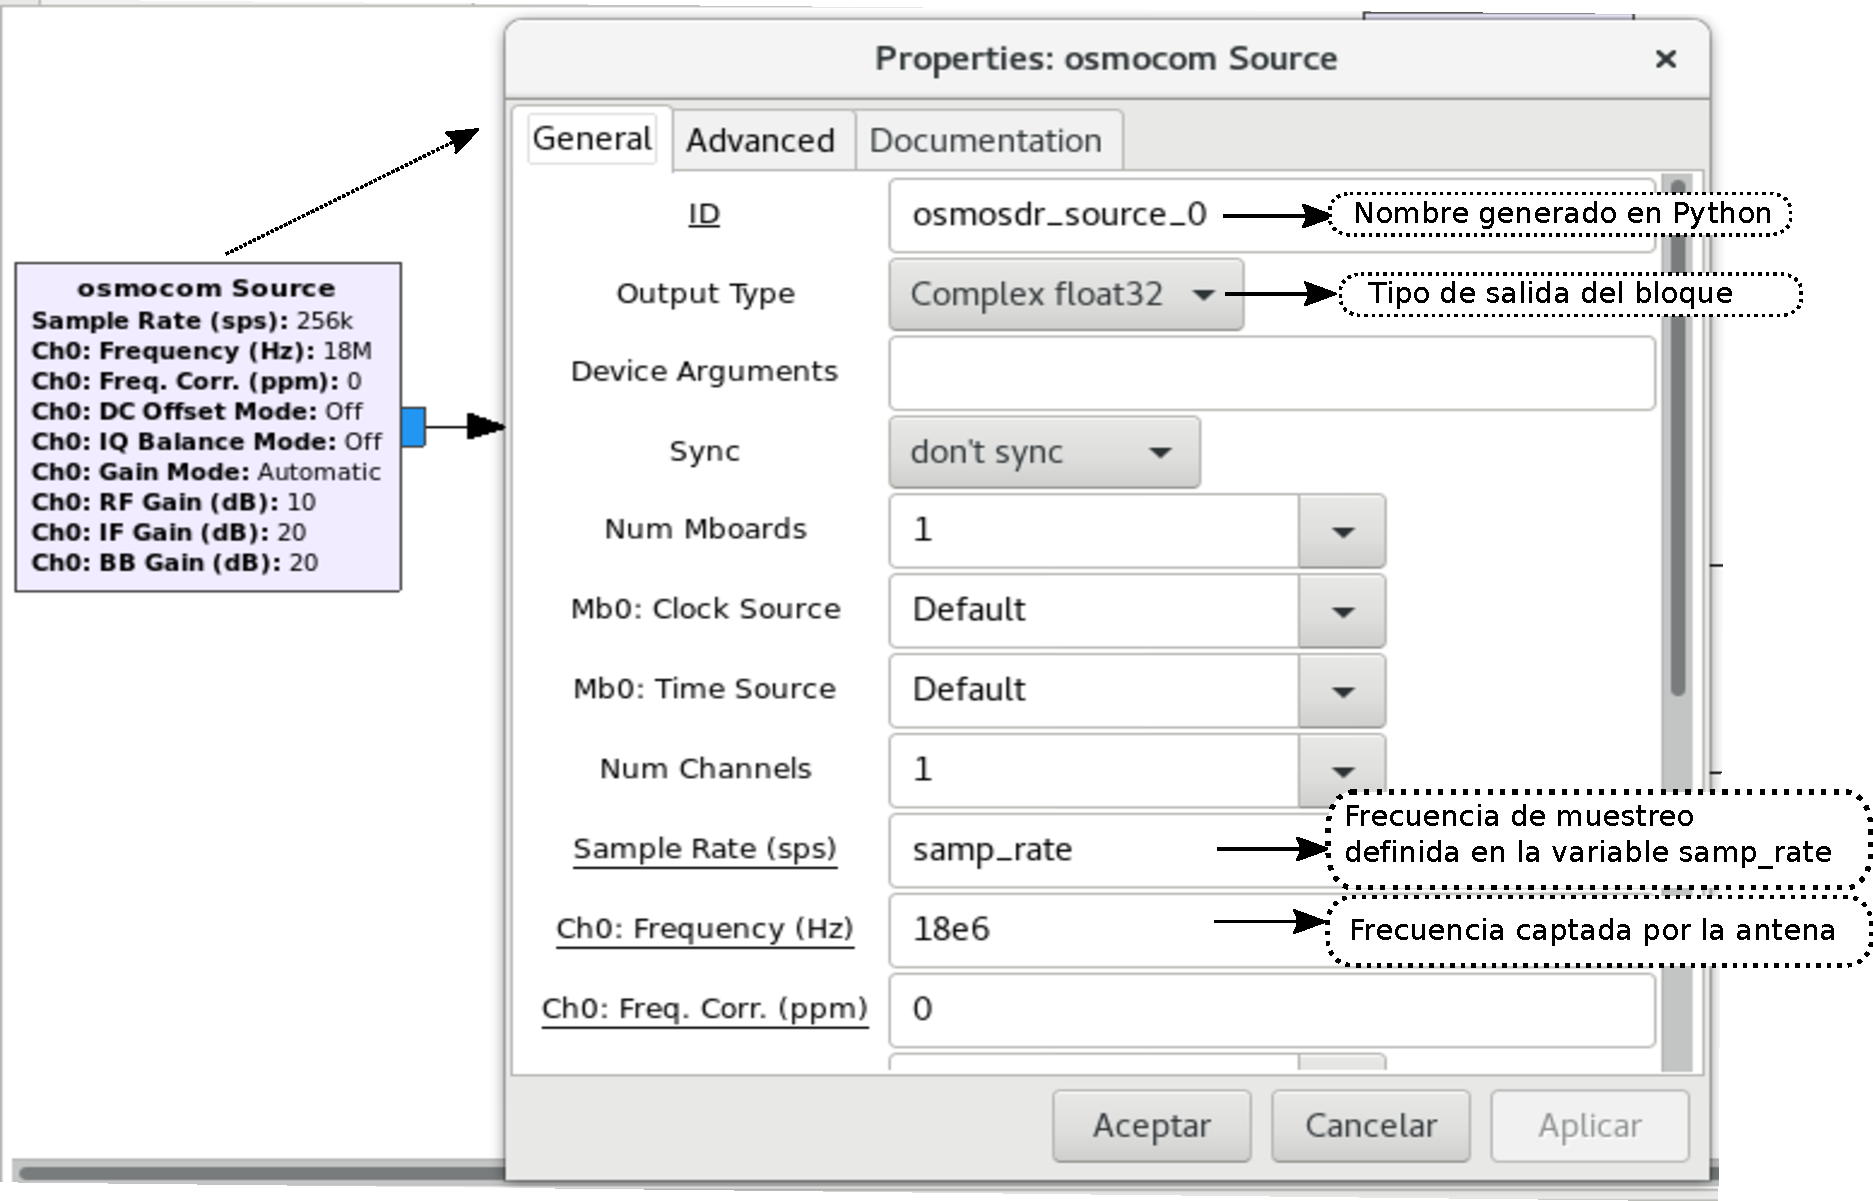
\includegraphics[width=\textwidth]{parte3/lab16/pdf/lab16_3.pdf}
\end{figure}

\end{frame}
%---------------------------------

\begin{frame}{Receptor AM}

\begin{figure}[H]
\centering
\vspace{-3mm}
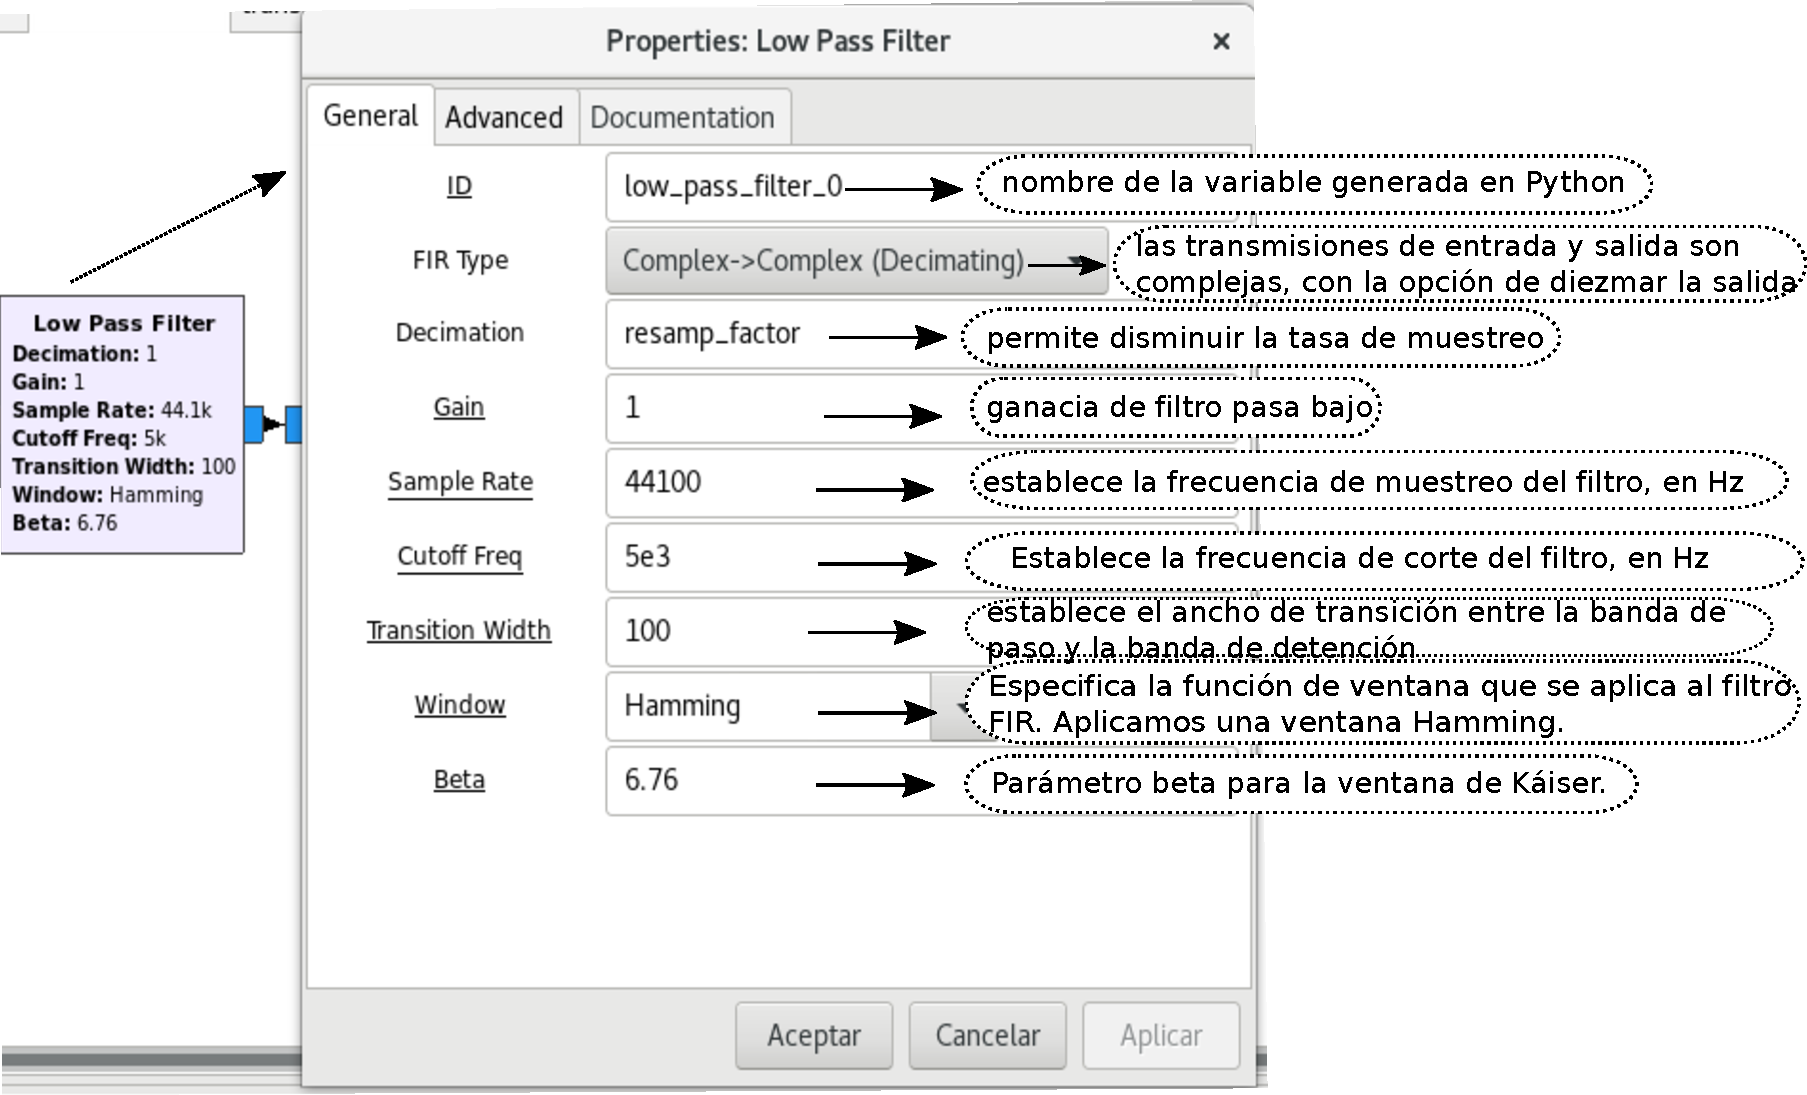
\includegraphics[width=\textwidth]{parte3/lab16/pdf/lab16_4.pdf}

\end{figure}

\end{frame}
%---------------------------------

\begin{frame}{Receptor AM}

\begin{figure}[H]
\centering
\vspace{-3mm}
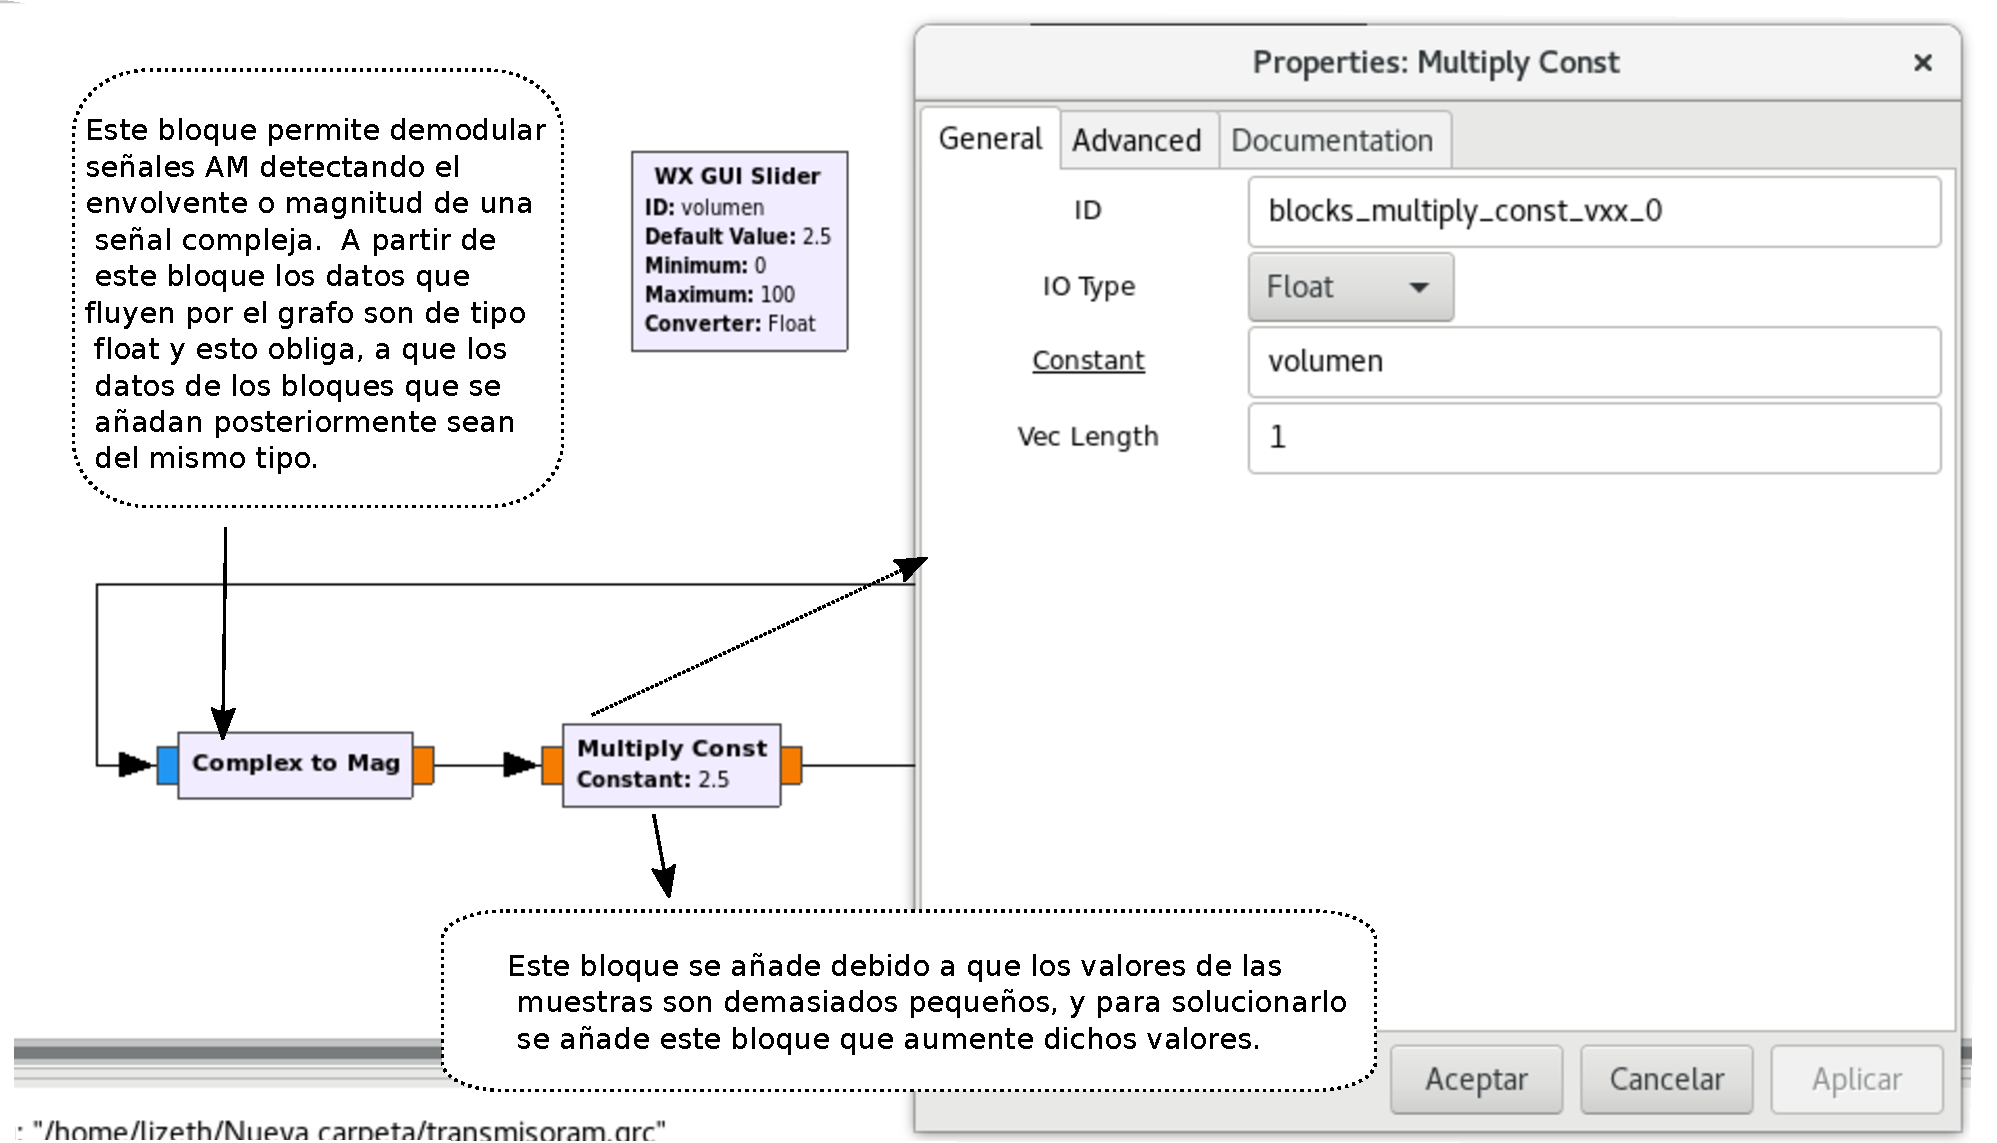
\includegraphics[width=\textwidth]{parte3/lab16/pdf/lab16_5.pdf}

\end{figure}

\end{frame}
%---------------------------------

\begin{frame}{Receptor AM}

\begin{figure}[H]
\centering
\vspace{-3mm}
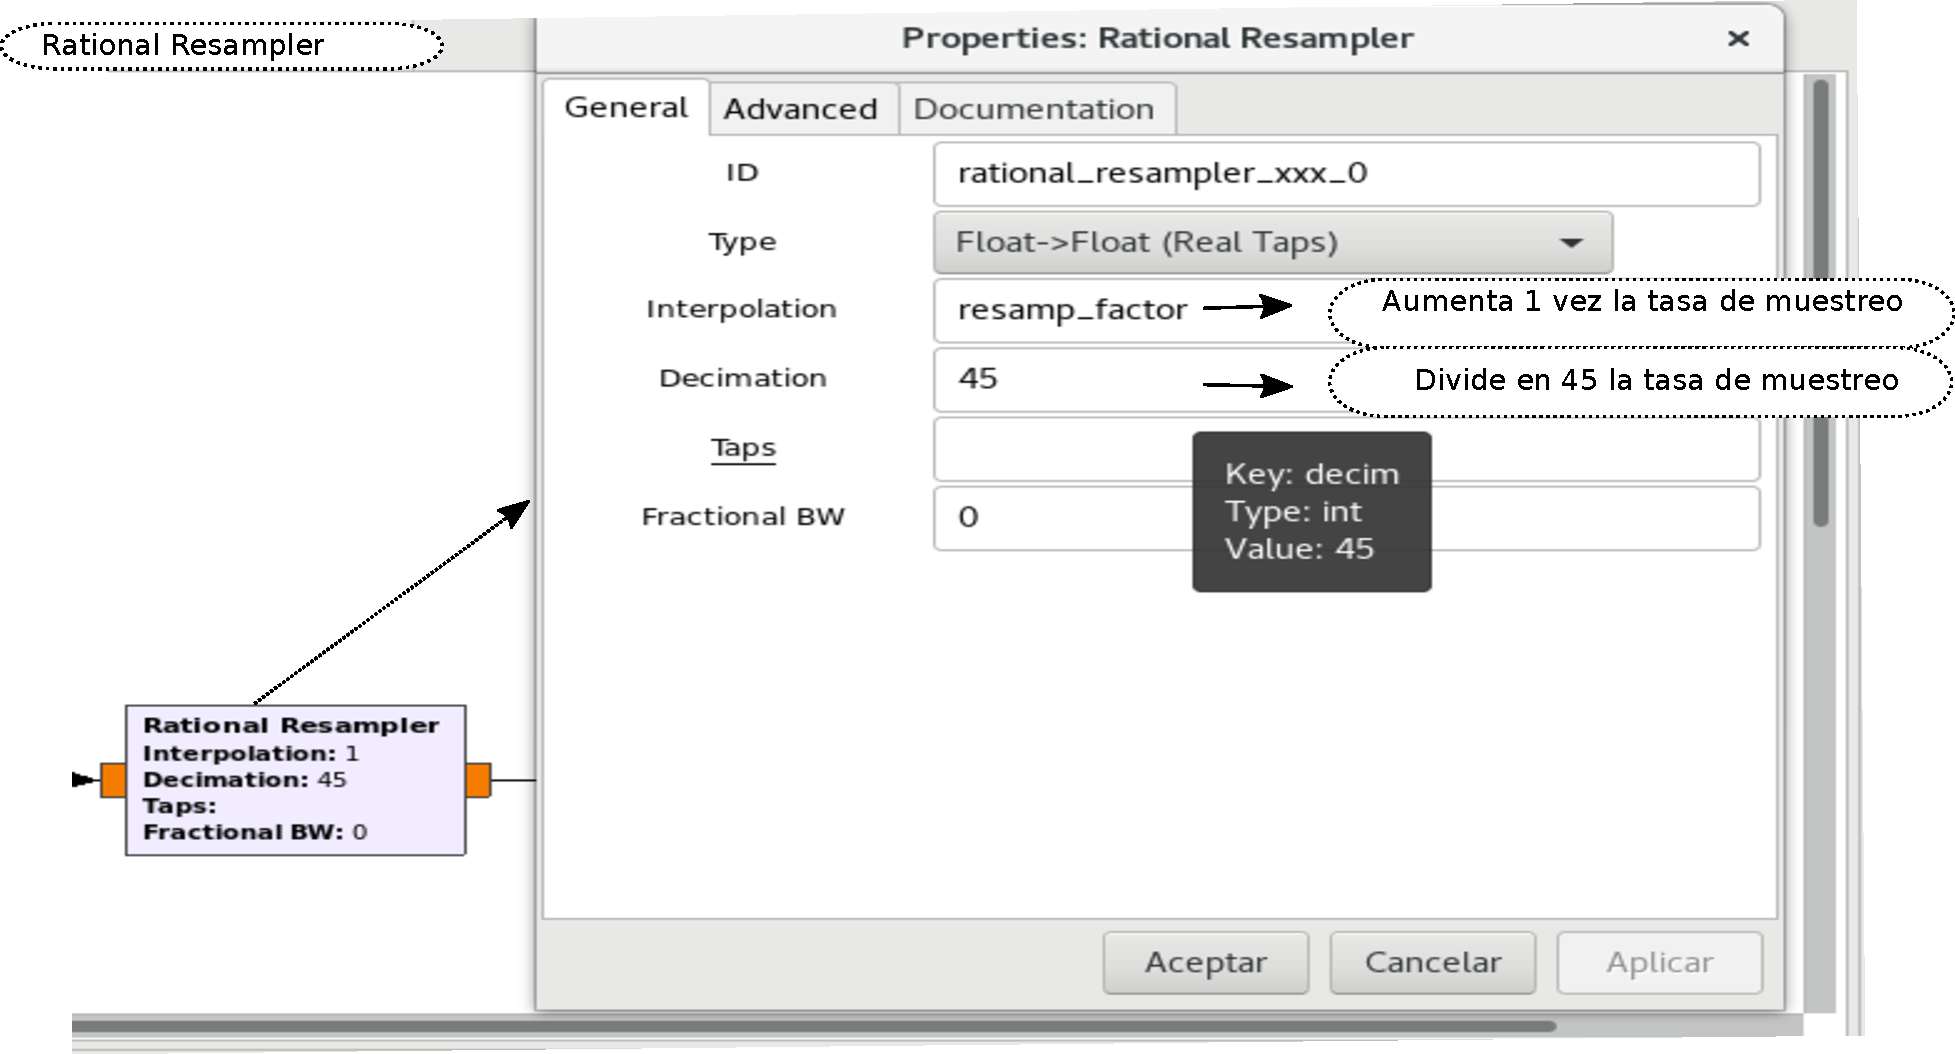
\includegraphics[width=\textwidth]{parte3/lab16/pdf/lab16_6.pdf}

\end{figure}

\end{frame}
%---------------------------------

\begin{frame}{Receptor AM}

\begin{figure}[H]
\centering
\vspace{-3mm}
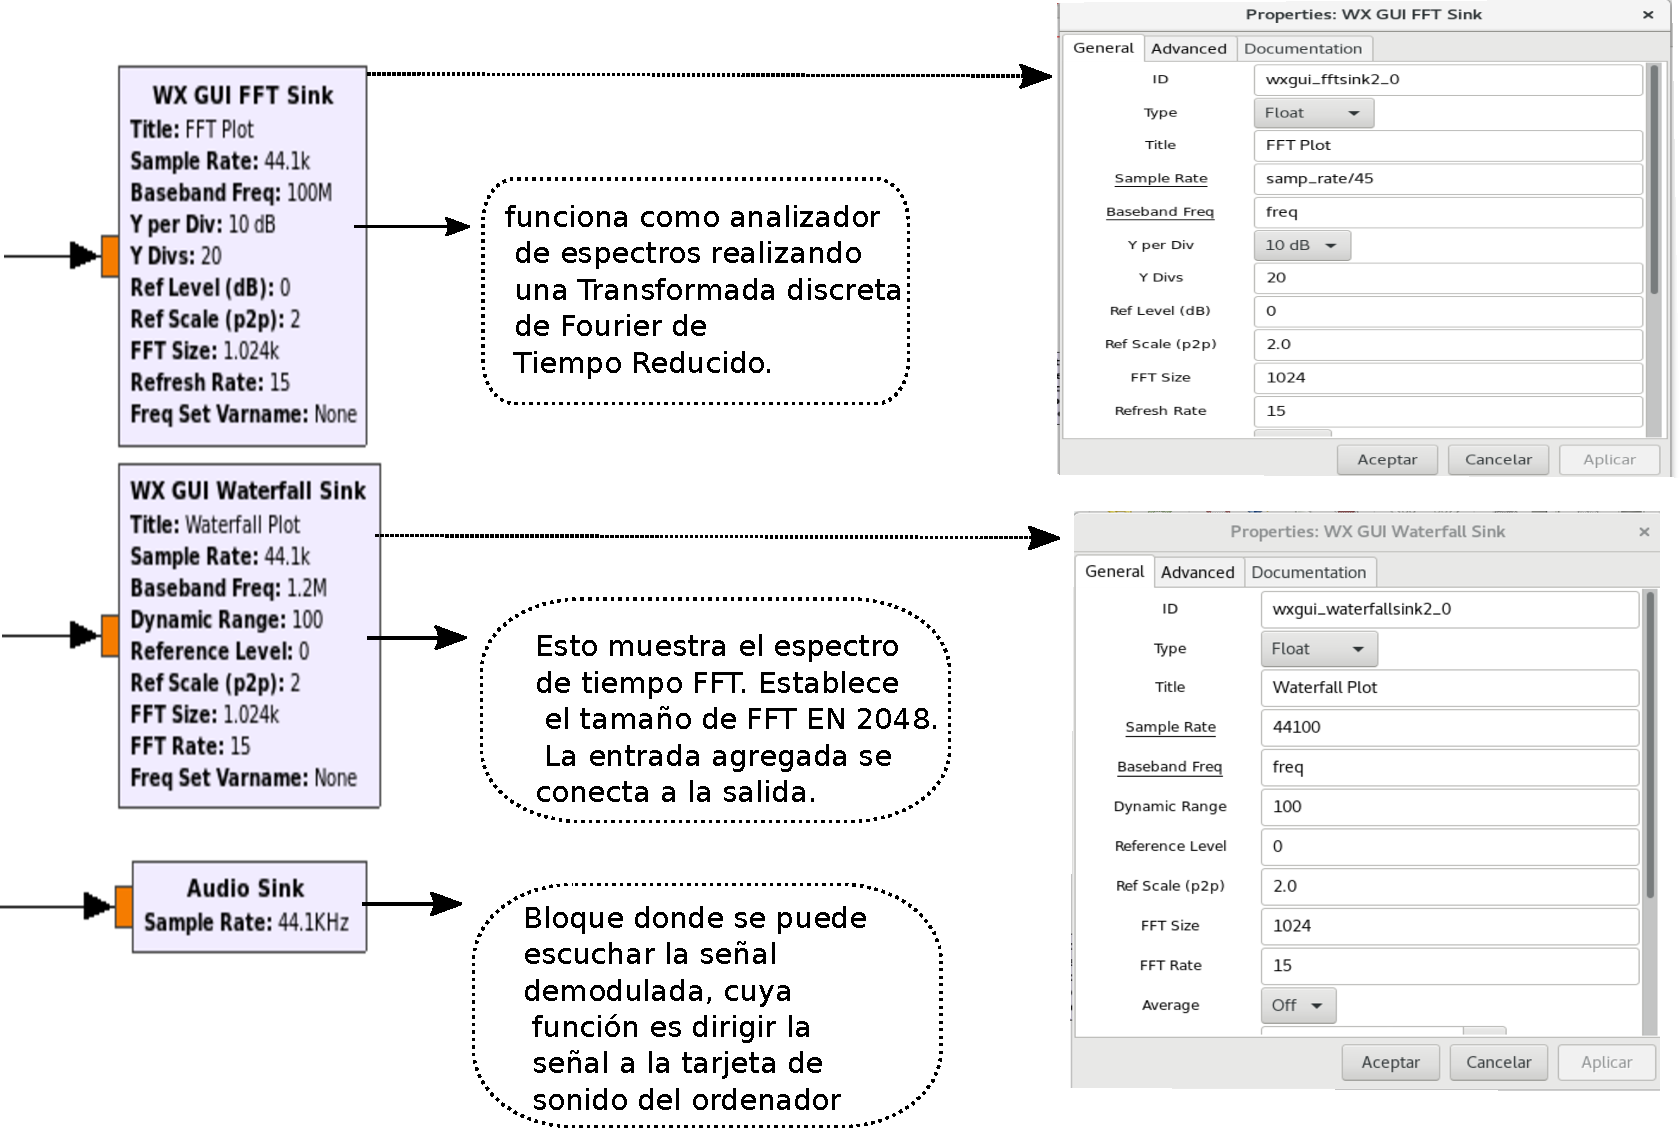
\includegraphics[width=\textwidth]{parte3/lab16/pdf/lab16_7.pdf}

\end{figure}

\end{frame}
%---------------------------------

\begin{frame}{Receptor AM}

\begin{figure}[H]
\centering
\vspace{-3mm}
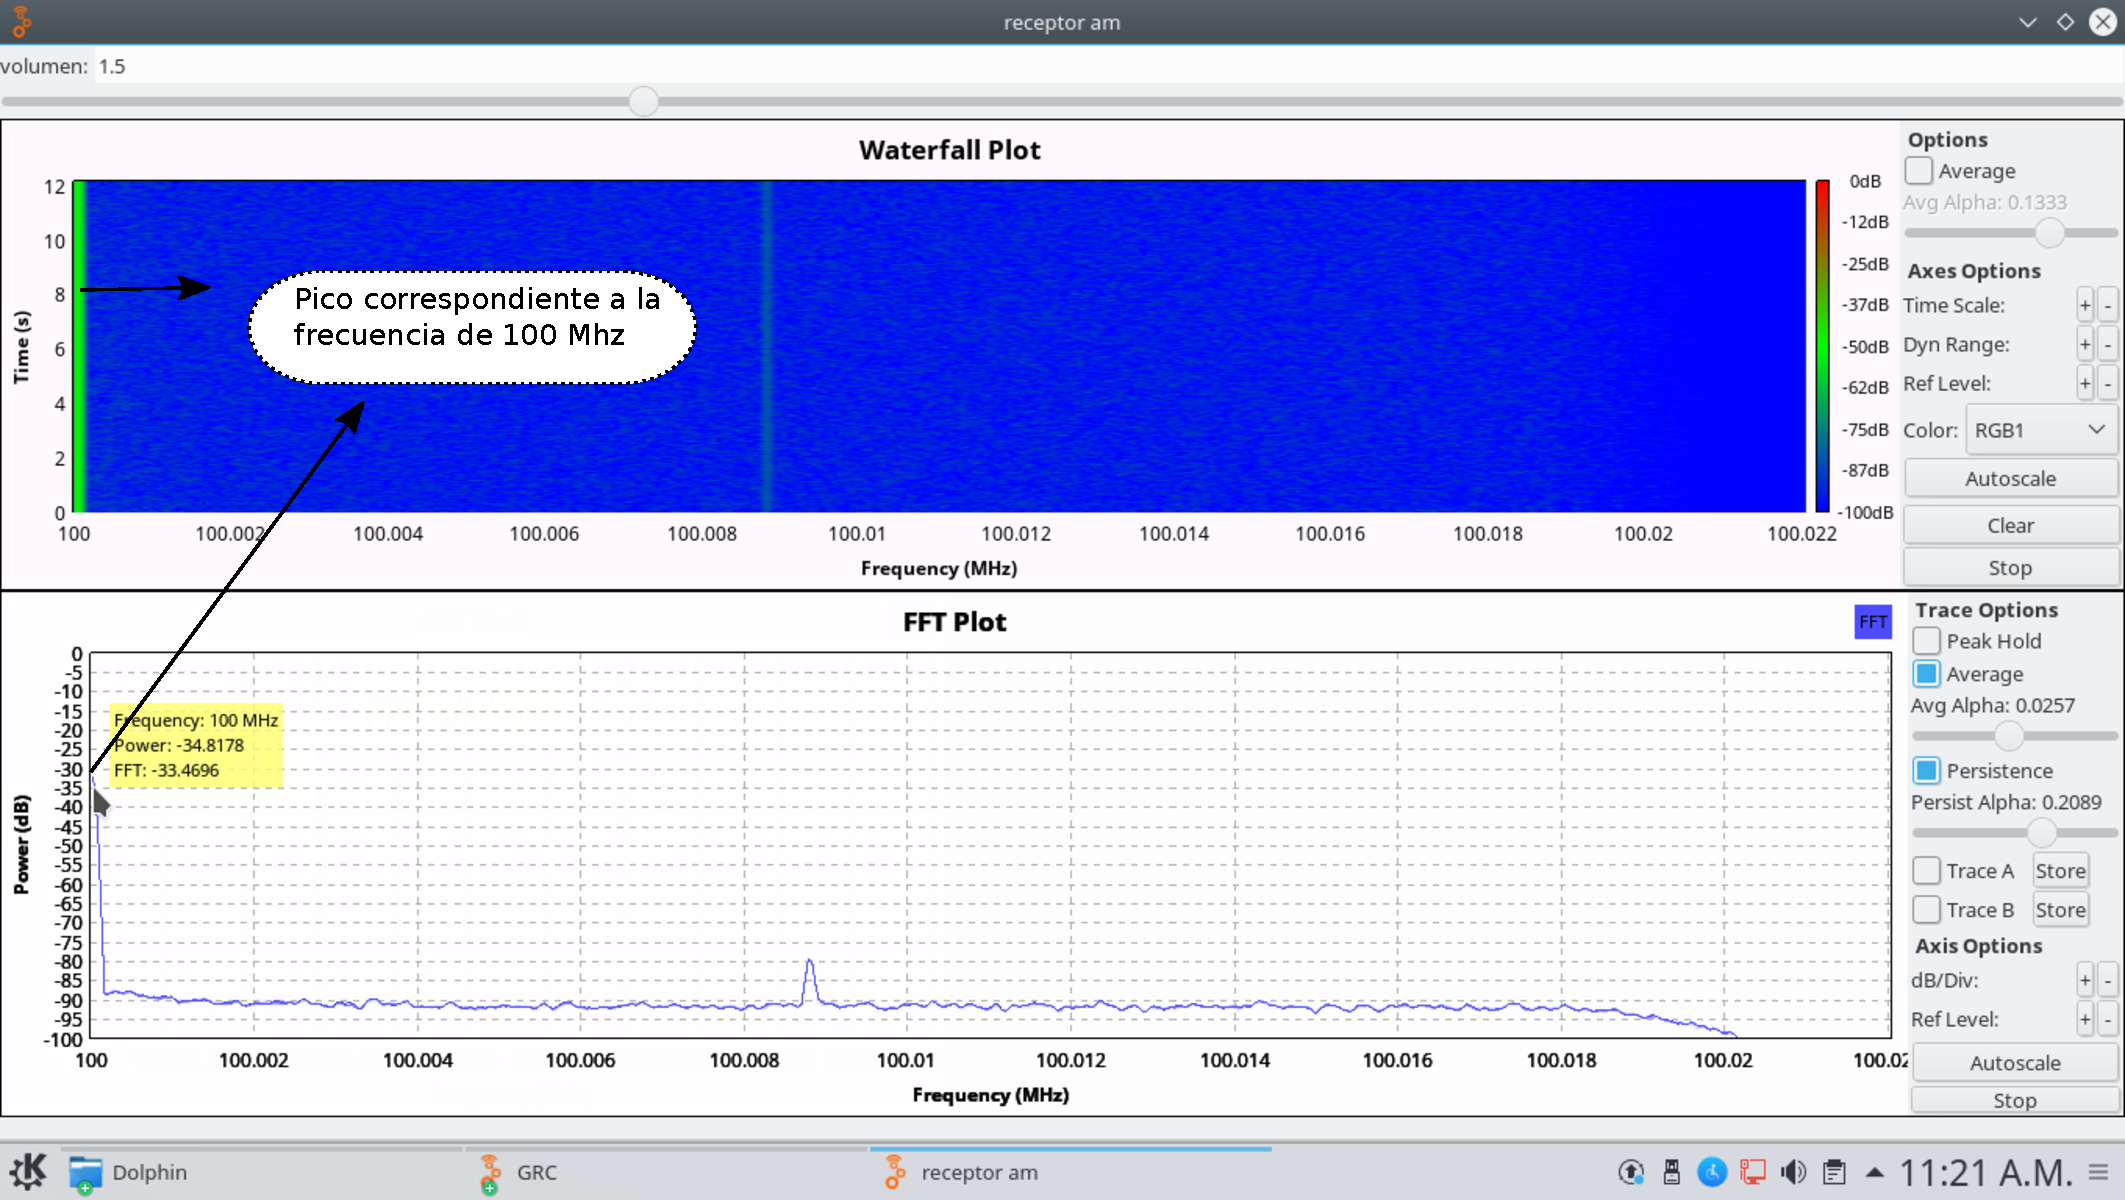
\includegraphics[width=\textwidth]{parte3/lab16/pdf/lab16_8.pdf}

\end{figure}

\end{frame}
%---------------------------------
